
\documentclass[10pt]{article}
\usepackage[margin=1in]{geometry}
\usepackage{graphicx}
\usepackage[font=small,labelfont=bf]{caption}


\setlength\textfloatsep{6pt plus 2pt minus 2pt}
\setlength\floatsep{6pt plus 2pt minus 2pt}
\setlength\intextsep{6pt plus 2pt minus 2pt}

\begin{document}
\section*{Is Florida getting warmer?}

Observed Pearson correlation between Year and Temp is \textbf{r = 0.533}. 
A permutation test with 10{,}000 shuffles yields a one-sided p-value
\textbf{$p < 10^{-4}$}. 

\medskip
\noindent The correlation is positive and highly significant, consistent with warming in Key West over the 20th century.

\begin{figure}[h]
\centering
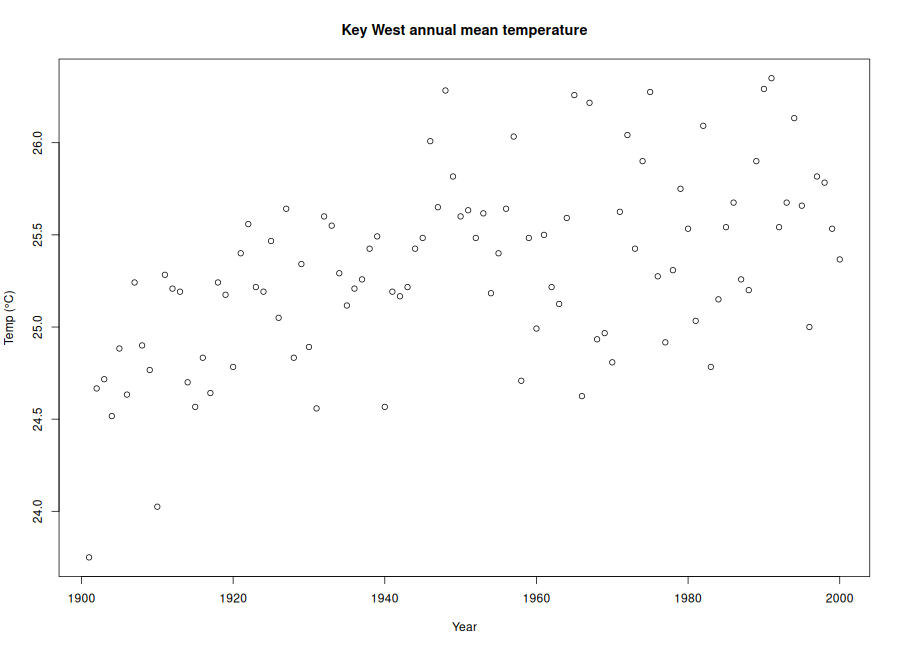
\includegraphics[width=.48\linewidth]{figs/scatter_year_temp.png}\hfill
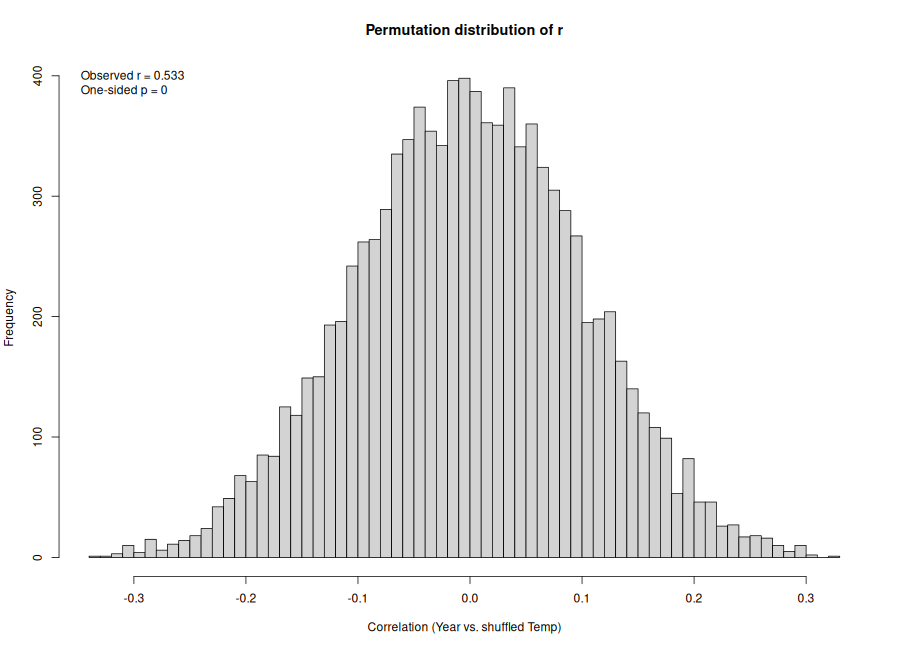
\includegraphics[width=.48\linewidth]{figs/permutation_correlations.png}
\caption{Left: Year vs. temperature. Right: permutation distribution (red line: observed $r$).}
\end{figure}
\end{document}
